\begin{figure}[!htbp]
\begin{center}

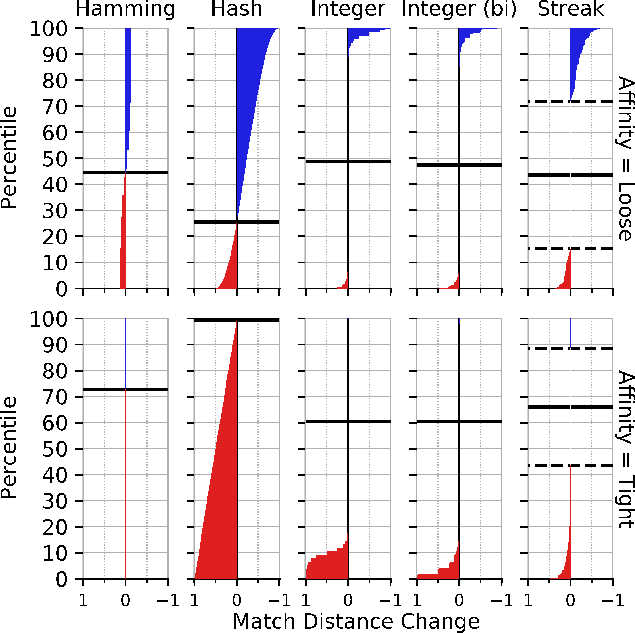
\includegraphics[width=\columnwidth]{img/mutational_step/bitweight=0dot5+seed=1+title=low-mutational-step+_data_hathash_hash=95a57768de56995a+_script_fullcat_hash=b9a24f3843e31e82+ext=}
\caption{
Distributions of mutation effects on match distance for loosely matched (pre-mutation match distance $> 0.5$) and tightly matched (pre-mutation match distance $< 0.01$) tag pairs.
Each distribution visualization arranges individually sampled observations of mutation outcome from an independently sampled tag pair (thin horizontal bars) vertically in descending order.
The $y$ axis can be interpreted as ranging from the \nth{0} percentile of outcomes (bottom) to \nth{100} percentile (top) with horizontal bar width showing the mutation effect size at a certain percentile.
Mutations that increase affinity are colored blue and mutations that decrease affinity are colored red.
Solid lines indicate the median between mutations that increase match distance and mutations that decrease match distance.
Dashed lines demarcate the boundaries between non-neutral and perfectly-neutral mutations.
Note that the $x$ axis is inverted so mutations increasing affinity fall to the right and mutations decreasing affinity fall to the left.
}
\label{fig:mutational_step_supp}

\end{center}
\end{figure}
